

% literature review


\chapter{Influence Maximization}\label{chap:lit}

\fancyhead[L]{\textit{Chapter 2. Influence Maximization}}

In this chapter, first we give an exhaustive definition of the influence maximization problem under the different diffusion models used for information propagation. Next, we present the different algorithmic approaches used for the non-adaptive greedy algorithm. Section \ref{sec:aim} gives a brief overview of the adaptive IM which is the main scope of the thesis. We introduce the adaptivity gaps and the different feedback models associated with the adaptive problem. A dedicated related works section for the AIM with the feedback models is presented. We also explore the work done on the unconventional non-monotone and DR-submodular models w.r.t adaptive IM. Finally, we discuss the commonly used techniques related closely to our work, and on which the thesis improves upon in section \ref{smp}.




\section{Main Definitions} \label{main}
We study the following dynamics consisting in multiple time steps. Given a graph $G = (V, E)$ as an input instance, we have a set $S \subseteq V$ of \emph{active nodes}\footnote{In this thesis, we will use the terms active and influenced nodes interchangeably.}, called the \emph{seed set}, which is responsible for the activation of nodes at the first time step, $t$. Furthermore, we have an underlying \emph{diffusion model} $M$, determining how the set of {active nodes}, at each time step, influences some {inactive nodes}, that become active at the next time step, $t+1$. The {\em influence function} $\sigma_{G, M} : 2^V \rightarrow \R_{\geq 0}$ associates to each possible initial seed set $S$, the expected value $\sigma_{G, M}(S)$ of nodes which are active at the end of the process.

The influence maximization problem can be formally defined as follows: 
given a budget of $k$ users, a graph $G$, and a diffusion model $M$, the goal is to select a seed set $S^*$ of $k$ users from $V$ in order to maximize the influence function, i.e., a set $S^*$ such that 
\begin{equation}
\sigma_{G,M}(S^*) = \argmax_{S\subseteq V:|S| \leq k} \sigma_{G,M}(S).
\end{equation}
Initially, all the nodes present in the seed set $S$ are active. As the nodes in the graph starts getting influenced, an inactive node $v$ will be activated by its active neighbours eventually, according to the considered diffusion model $M$. A node $u \in V$ is said to be the {\em neighbour} of $v$ if there is an edge $(u,v)\in E$. The diffusion process comes to a halt when there are no more activations. One classic example of influence function is the expected number of influenced nodes.

The main objective of the IM problem is to find a seed set of at most $k$ nodes that maximizes the value of $\sigma_{G,M}$ at the end of the diffusion process. However, maximizing $\sigma_{G,M}$ is often a computationally hard problem. To overcome this issue, one can resort to an {\em $\alpha$-approximation algorithm}, that computes in polynomial time an approximate optimal seed set $S$ with an {\em approximation factor} of $\alpha\leq 1$, i.e., a seed set $S$ such that $\sigma_{G,M}(S)\geq \alpha\cdot \sigma_{G,M}(S^*)$. Most of the approximation algorithms considered for the IM problem require that function $\sigma_{G,M}$ verify two desirable properties: \emph{monotone} and \emph{submodular}. A monotone function ensures that adding nodes to the seed set will not reduce the value of $\sigma_{G,M}$, whereas submodular means that the marginal gain of adding a node to the seed set does not increase as the size of the seed set increases. In particular, $\sigma_{G,M}$ is {\em monotone} if, for any $S\subseteq V$ and for any $x\in V\setminus S$, we get $\sigma_{G,M}(S)\leq \sigma_{G,M}(S\cup\{x\})$. Furthermore, $\sigma_{G,M}$ is {\em submodular} if, for any $S,P\subseteq V$ such that $S\subseteq P$ and  for any $x\in V\setminus P$, we get $\sigma_{G,M}(P\cup\{x\})-\sigma_{G,M}(P)\leq \sigma_{G,M}(S\cup\{x\})-\sigma_{G,M}(S)$. In subsection \ref{nonada_sec}, we will formally describe a greedy approximation algorithm for the non-adaptive IM that exploits these properties to guarantee a good approximation ratio. 






\section{Diffusion Models}

The design of diffusion models is an integral aspect of the IM problem. There are two kinds of diffusion processes: \emph{progressive} and \emph{non-progressive}. In the progressive model, once a node is  activated, deactivation is impossible. In contrast, the non-progressive model allows an activated node to be deactivated later in the diffusion process. Even-Dar et al.~\cite{Even-Dar2007} studied the IM problem by exploiting the \emph{Voter Model} \cite{Clifford1973}, which is an example of a non-progressive case. In this thesis, we restrict our study only to progressive models. 

Models can also be \emph{time-unbounded} and \emph{time-bounded}. In time-unbounded models, termination occurs when the node activation comes to a halt. Whereas, the time-bounded models have a separate time parameter for the completion of an ongoing diffusion process. Most of the previous work and the works in this thesis are mainly focus on time-unbounded models. Some examples of time-unbounded models are the independent cascade, linear threshold and \emph{triggering}. For AIM and this thesis, only the IC model is considered, however, there is a section dedicated to the experiments on LT. The following subsections explain the IC, LT and triggering model in details.


\begin{figure}[!h]
\centering
\begin{subfigure}{0.3\textwidth}
    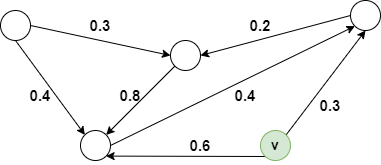
\includegraphics[width=\textwidth]{GSSI_thesisProposal/figures/ic1.png}
    \caption{At $t=0$}
    \label{fig:ic1}
\end{subfigure}
\hfill
\begin{subfigure}{0.3\textwidth}
    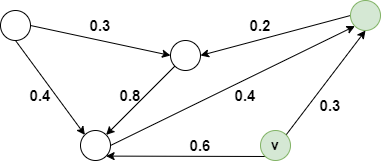
\includegraphics[width=\textwidth]{GSSI_thesisProposal/figures/ic2.png}
    \caption{At $t=1$}
    \label{fig:ic2}
\end{subfigure}
\hfill
\begin{subfigure}{0.3\textwidth}
    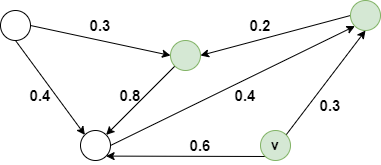
\includegraphics[width=\textwidth]{GSSI_thesisProposal/figures/ic3.png}
    \caption{At $t=2$}
    \label{fig:ic3}
\end{subfigure}
\caption{Diffusion process under the independent cascade at several time steps.}
\label{fig:cascade}
\end{figure}

\begin{figure}[!h]
\centering
\begin{subfigure}{0.3\textwidth}
    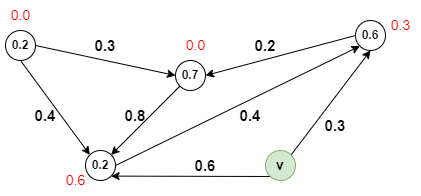
\includegraphics[width=\textwidth]{GSSI_thesisProposal/figures/lt1.png}
    \caption{At $t=0$}
    \label{fig:lt1}
\end{subfigure}
\hfill
\begin{subfigure}{0.3\textwidth}
    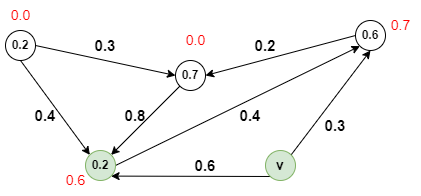
\includegraphics[width=\textwidth]{GSSI_thesisProposal/figures/lt2.png}
    \caption{At $t=1$}
    \label{fig:lt2}
\end{subfigure}
\hfill
\begin{subfigure}{0.3\textwidth}
    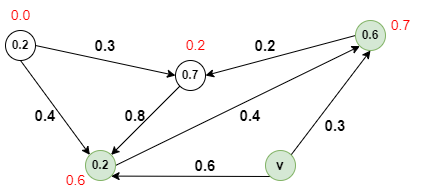
\includegraphics[width=\textwidth]{GSSI_thesisProposal/figures/lt3.png}
    \caption{At $t=2$}
    \label{fig:lt3}
\end{subfigure}
\caption{Diffusion process under the linear threshold at several time steps.}
\label{fig:linear}
\end{figure}





\subsection{Independent Cascade Model}

In the IC model, we have an {\em influence graph}  $G=(V=[n],E,(p_{uv})_{(u,v)\in E})$, where edges are directed and $p_{uv}\in [0,1]$ is an {\em activation probability} associated to each edge $(u,v)\in E$. Given a set of {\em seeds} $S\subseteq V$ which are initially \emph{active}, the diffusion process in the IC model is defined in $t\geq 0$  discrete steps as follows: (i) let $A_t$ be the set of active nodes which are activated at each step $t\geq 0$; (ii) $A_0:=S$; (iii) given a step $t\geq 0$, for any edge $(u,v)$ such that $u\in A_t$, node $u$ can activate node $v$ with probability $p_{uv}$ independently from any other node, and in case of success, $v$ is included in $A_{t+1}$; (iv) the diffusion process ends at a step $r\geq 0$ such that $A_{r}=\emptyset$, i.e., no more nodes in the graph can be activated. The size of $\bigcup_{t\leq r} {A_t}$, i.e. the number of nodes activated/reached by the diffusion process, is the {\em influence spread}. Figure \ref{fig:cascade} shows the influence unravelling at different time steps for the IC model.

We point out that the activation of an edge $(u,v)$ is a random event determined by the outcome of a coin toss that gives \textbf{head} with probability $p_{uv}$. Before the start of the diffusion process, the biased coin is flipped for every edge in the graph $G$. By looking at the influence probabilities; one can conclude whether a node $v$ will be active after the termination of the cascade process or not.

The above diffusion process can be equivalently defined as follows. The {\em live-edge graph} $\bm L=(V,\bm L(E))$ is a random graph of $G$, such that each edge $(u,v)\in E$ is included in $\bm L(E)$ with probability $p_{uv}$, independently from the other edges, i.e., $\mathbb{P}[\bm L=L]=\prod_{(u,v)\in L}p_{uv}\prod_{(u,v)\in E\setminus L}(1-p_{uv})$. 

With a little abuse of notation, we may denote $L(E)$ with $L$. Given $L\subseteq E$, let $R_L(S):=\{v\in V:\text{there exists a path from $u$ to $v$ in $L$ for some $u\in S$}\}$, i.e., the set of nodes reached by $S$ in the graph $L$. Informally, if $S$ is the set of seeds, and $L$ is a realisation of the live-edge graph, $R_L(S)$ equivalently denotes the set of nodes which are reached/activated by the above diffusion process. Let $\sigma_L(S):=|R_L(S)|$ denote the {\em influence spread} generated by the set of seeds $S$ if the realised live-edge graph is $L$, and let $\sigma(S):=\mathbb{E}_{ L}[\sigma_{{L}}(S)]$ be the {\em expected influence spread} generated by $S$. For a clear visualization of the realisations of a live-edge graph, refer to figure \ref{fig:real}.

Kempe et al.~\cite{Kempe2003} shows that finding the set of influential nodes maximizing the influence function in the IC model is NP-hard, and they use a reduction to the {\em Maximum Coverage} problem. A particular model of IC is that of \emph{Weighted Cascade}. In such a model, each influence probability is defined as $p_{uv}=1/d_{in}(v)$, where $d_{in}(v)$ is the in-degree of $v$. In this process, a node is equally influenced by each of its neighbours. 

Other models assume that the influence probabilities are not known. Saito et al.~\cite{Saito2008} predict the influence probabilities by using the \emph{Expectation Maximization} algorithm to compute the diffusion probabilities of all the edges in $G$,  repeatedly, to maximize the objective function. Goyal et al.~\cite{Goyal2010} developed a learning algorithm which takes as input a social graph and the \emph{Action Log}, that reports the actions performed by all the nodes. 


\begin{figure}[!h]
\centering
\begin{subfigure}{0.3\textwidth}
    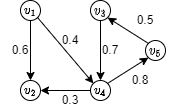
\includegraphics[width=\textwidth]{GSSI_thesisProposal/figures/real_1.png}
    \caption{Graph G}
    \label{fig:real_1}
\end{subfigure}
\hfill
\begin{subfigure}{0.3\textwidth}
    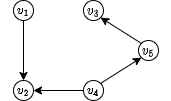
\includegraphics[width=\textwidth]{GSSI_thesisProposal/figures/real-2.png}
    \caption{Realisation $\phi_1$}
    \label{fig:real_2}
\end{subfigure}
\hfill
\begin{subfigure}{0.3\textwidth}
    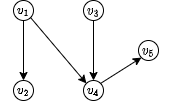
\includegraphics[width=\textwidth]{GSSI_thesisProposal/figures/real-3.png}
    \caption{Realisation $\phi_2$}
    \label{fig:real_3}
\end{subfigure}
\caption{A graph $G$ and two of its possible realisations.}
\label{fig:real}
\end{figure}


\subsection{Linear Threshold (LT) Model} \label{sec:lt}

Granovetter~\cite{Granovetter1978} introduced the \emph{Linear Threshold model}, where he proposed a diffusion model in which each node $v$ becomes active if the weighted sum of its active neighbours reaches a certain threshold. More formally, the model takes as input a graph $G$, the seed set $S$, and an edge weight $W_{u,v}$ for any edge $(u,v)\in E$. Before the diffusion starts, a \emph{threshold value} $\theta_v$ is picked uniformly at random in the interval $[0,1]$ by each node $v\in V$, independently from the other nodes.

At each time step $t$ a node $v$ will get activated if the summation of edge weights of its active neighbours reach the threshold value $\theta_v$, i.e.,  
\begin{equation}
\sum_{(u,v)\in E: u\text{ is active}} W_{u,v}  \geq \theta_u
\end{equation}
The process proceeds in several time steps and terminates when no more activations are possible. Figure \ref{fig:linear}, shows the steps of information diffusion in this model. The number inside the node indicates its threshold. A red counter on the side indicates the current active edge weight of a node. If the number in the red counter equals or exceeds the threshold of a specific node, then the node gets activated. Kempe et al.~\cite{Kempe2015} showed that finding the set $S$ maximizing the influence function in the LT model is also NP-hard, and they use a reduction to the {\em Vertex Cover} problem.  

A \emph{Generalized Threshold Model} can be designed by removing the linearity from LT. The model follows the same structure as LT. However, $v$ now relies upon an arbitrary {\em monotone threshold function} $f_v$ which maps the subsets of $v$’s neighbours into the interval $[0,1]$, with $f_v(\emptyset) = 0$. Let $N$ represent the set of neighbours of $v$ that are active at time step $t-1$. Node $v$ becomes active at time step $t$ if and only if $f_v(N) \geq \theta_v$. The LT model is a special case of the generalized threshold model. The threshold function of the LT model takes the following form:
\begin{equation}
f_v(N) = \min\left(1, \sum_{u \in N} W_{u,v}\right).
\end{equation}
The General Threshold model is {\em submodular} if each function $f_v$ is submodular. If this model is not submodular, its analysis may be intractable. 

\subsection{Triggering Model}

The IC and the LT are specialized cases of the \emph{triggering} model also introduced by Kempe et al.~\cite{Kempe2015}. In this model, instead of having a threshold value, a node $v$ has a quiescent subset $T_v$, called the \emph{triggering set}, which affects the state of $v$. Initially, the process starts with a seed set $S$, and each node $v$ chooses a triggering set $T_v$ independently from each other, according to some distribution over the subsets of its neighbours. An inactive node $v$ can be activated at time step $t$, if it has an active neighbour $u$ in $T_v$ at time step $t-1$.

Another way to think of this process is by considering the \emph{live-edge} technique. Edges of a graph $G=(V, E)$ can be either {live} or {blocked}. If a node $u$ is present in the triggering set $T_v$ of $v$, the edge $(u,v) \in E$ will be declared as live and claimed to be blocked otherwise. So, $v$ is reachable from the seed set $S$ by traversing a path made entirely out of live edges. The influence function $\sigma$ is shown to be submodular in the triggering model. 





\section{Non-Adaptive Influence Maximization}\label{nonada_sec}



The {\em non-adaptive influence maximization} is a computational problem, where given an influence graph $G$ and an integer $k\geq 1$, we are asked to find a set of seeds $S\subseteq V$ with $|S|\leq k$ such that $\sigma(S)$ is maximized. Without loss of generality, we assume that $k\in [n]$, and since the objective function is monotone, $|S|=k$ for any solution of $S$.

Kempe et al.~\cite{Kempe2003,Kempe2015} showed that function $\sigma$ is monotone and submodular, therefore the following greedy algorithm achieves a $1-\frac{1}{e}$ approximation factor. Algorithm \ref{algo:non} is as follows: (i) start with an empty set of seeds $S:=\emptyset$; (ii) at each iteration $t\in [k]$, add to $S$ the node $v$ that maximizes the expected influence spread $\sigma(S\cup \{v\})$. Note that the greedy algorithm requires at each iteration to compute the value of function $\sigma$, for some set of seeds.


\begin{algorithm}[ht]
	\caption{Non-Adaptive algorithm}
	\label{algo:non}
	\begin{algorithmic}[1]
		\REQUIRE an influence graph $G$;
		\STATE $S$ $\leftarrow$ $\emptyset$;
		\WHILE{{$|S| < k$}}
		\STATE $v^* \leftarrow \argmax_{v \in V \setminus S} (\sigma(S \cup \{v\})-\sigma(S))$;
		\STATE $S \leftarrow S \cup \{v^*\} $;
		\ENDWHILE
		\RETURN $S$;
	\end{algorithmic}
\end{algorithm}





\medskip

By using the fact that $\sigma$ is a monotone submodular function with $\sigma(\emptyset)=0$, the results of Nemhauser and Wolsey~\cite{Company1978} on submodular function approximation imply that algorithm \ref{algo:non} will always produce a solution guaranteeing at least $1-[(k-1)/k]^k\geq 1-1/e$ times the optimal value, where $e\simeq 2.71$ is the {\em Nepero number}.

At each step of algorithm \ref{algo:non}, we are required to compute the value $\sigma(S\cup\{v\})$ for any node $v\in V\setminus \{v\}$ to find the local optimal influence function, but this has been shown to be computationally intractable as it is $\#P$-hard~\cite{Chen10}. However, standard Chernoff bounds allow us estimate the value of $\sigma$ through a polynomial number of Monte-Carlo simulations by introducing an arbitrarily small additive error $\epsilon>0$, which depends on the number of simulations~\cite{Kempe2015}. In the reminder of the thesis, we will omit the additional term $\epsilon$ to avoid unnecessary complicated formulas (except for the experimental part, where we set $\epsilon=0.05$). We will refer to this algorithm as the \emph{non-adaptive greedy algorithm} in this thesis.

The two most widely studied non-adaptive IM algorithms are classified under the following categories: i) Monte-Carlo simulations-based approach \cite{Kempe2003} and, ii) Heuristic-based approach \cite{Borgs2014}.


\paragraph{Monte-Carlo simulation-based approach.} Kempe et al.'s non-adaptive greedy algorithm is an effective and simple algorithm that produces near optimal solution with a theoretical guarantee due to submodularity. They use Monte Carlo simulations to overcome the drawback of $\#P$-hard complexity. A Monte Carlo simulation is used to predict a model, by assigning a set of generated values based on a probability distribution to the uncertain variables. The simulations are computed independently on all the randomly generated values to obtain the results, which are then averaged to arrive at an estimate. Multiple instances of the graph $G$ are created and the number of reachable nodes $R(S)$ are computed for each of the generated instances. The value of $R(S)$ is averaged and the expected number of reachable nodes by S is $\sigma(S)$.

Nevertheless, the overhead cost that is incurred with a simple greedy algorithm is huge, because for each candidate seed node, the greedy algorithm simulates the influence cascade for estimating the influence increment. The number of Monte Carlo simulations required by the greedy algorithm is $O(mR)$, $O(m)$ is the time required for each simulation and $R$ is the number of simulations required ($R \approx 10000$ \cite{Kempe2003} for a good estimate). The resulting time complexity for the greedy algorithm is $O(kmnR)$, where $k$ is the total number of iterations, and $O(n)$ is the number of simulations for each iteration. 

Leskovec et al.~\cite{Leskovec2007} introduced the CELF algorithm which uses ``lazy-forward" optimization to improve on the time complexity for over 700 times by avoiding unnecessary simulations. They studied the structural property of social networks to find that real networks are mostly power-law graphs, which means majority of the nodes have a small influence. The algorithm maintains a priority queue to store the marginal influence of a node $v$ and the iteration number where it was computed. A node with a small influence in its previous iterations will not have a bigger marginal gain due to submodularity. Hence the simulation omit these nodes from its calculation without affecting the effectiveness of the algorithm.

The CELF algorithm was further improved by Goyal et al.~\cite{Goyal11} with CELF++ which ran $35\%-55\%$ faster than CELF. Other simulation based approaches include that of Cheng et al.~\cite{DBLP:conf/cikm/ChengSHZC13} to reduce the number of computations of CELF. Another simulation based paper was by Ohsaka et al.~\cite{DBLP:conf/aaai/OhsakaAYK14}, where they prune the number of BFSs required for reachability tests by reducing the number of vertices visited during each BFS. However, Monte Carlo simulations are computationally expensive and has scalibility issues when the graph starts to grow. 

\paragraph{Heuristic-based approach.}

In order to tackle with the expensive computations and large-scale networks,
Chen et al.~\cite{DBLP:conf/kdd/ChenWY09} used the degree discount technique which reduces the running time but has a much lower efficiency compared to the Monte Carlo approach. Borgs et al.~\cite{Borgs2014} introduced the \textit{reverse sampling technique (RIS)} and utilizes the concept of \textit{reverse reachable (RR) sets} and \textit{Random RR sets}. An instance $g$ of graph $G$ is generated by using the value of $p_{(uv)}$ to add edges in $g$ between nodes $u$ and $v$ of $g$. The RR set for a node $u$ in $g$ is the set of nodes that have a directed path to $u$ in $g$. Due to the randomness of generating $g$ using the probability on edges, we have a distribution $\mathcal{G}$ of $g$. To generate a random RR set on $g$, the instance $g$ is randomly sampled from $\mathcal{G}$. 

The idea behind Borgs et al.'s algorithm RIS, is to generate a large set of random RR sets, denoted as $\mathcal{R}$. Using the greedy maximum coverage algorithm from \cite{Vazirani} the goal is to find a seed set $S^*$ of size $k$ which covers the maximum number of RR-sets, this implies that $S^*$ will have the maximum expected spread over all the size $k$ seed sets of $G$. Borgs et al.'s technique reduces the estimation of a large number of node sets hence reducing the overhead time complexity induced by simulation based approaches. To calculate the number of RR sets that needs to be generated, RIS proposed a predefined threshold value $\tau$. Defining a proper $\tau$ value results in a seed set $S$ being generated at almost linear time complexity with an approximation ratio of $(1-\frac{1}{e}-\epsilon)$. The RIS still has some overhead cost due to the dependency of $\tau$ on the number of nodes and edges examined.

Tang et al.~\cite{Tang2014} provided an improved version of the RIS algorithm called $TIM^+$. They mainly cut down the threshold cost by replacing it with a predefined constant $\theta$. TIM removes the dependency from the edges, and uses Chernoff bounds to estimate the value for $\theta$. The estimated time complexity of the $TIM^+$ algorithm is $O((k+l)(m+n)\text{log} n/\epsilon^2)$, where $l$ is a constant and is set to $1$. For the experimental part of the thesis (section \ref{exp}), we use $TIM^+$ as the base non-adaptive greedy algorithm.
Tang et al.~\cite{Tang15} further improved on the efficiency of $TIM^+$ with the IMM algorithm by bounding the size of $\mathcal{R}$ using a martingle approach.

More improvements on the IMM algorithm was brought by Nguyen et al.~\cite{Nguyen16}, Huang et al.~\cite{Huang}, Tang et al.~\cite{Tang2019} where they curb the excessive generation of RR sets when the value of $k$ is large. They work with the \textit{Stop-and-Stare} algorithm \cite{Nguyen16}, where they set a stopping time limit $T$. The sampling process is stopped when $T$ is reached and the algorithm checks if the seed set $S$ fulfils the $(1-1/e-\epsilon)$-approximation. Once the current $S$ reaches the approximation, the algorithm terminates. 


The heuristic-based approach has better scalibility and time complexity, but lacks in the department of performance guarantees that the simulation-based approach can provide.

 


\section{Adaptive Influence Maximization} \label{sec:aim}


\subsection{Adaptive Maximization} 


Golovin and Krause~\cite{Golovin2011} studied the {\em Adaptive Maximization (AM)} setting, and later applied it to the context of Influence Maximization by introducing its adaptive version. The general problem of AM is defined as follows: consider a graph $G=(V,E)$ and a set of states $O = \{alive, dead\}$. Each edge $e \in E$ is in one of the possible states, so that the state of the edges can be represented using a function $\phi: E \mapsto O$, called the \emph{realisation}. Hence, we can state that $\phi(e)$ is the state of $e$ under realisation $\phi$. A random variable $\Phi$ taking values from all the possible realisations, according to a given probability distribution, is called a {\em random realisation}. For a given realisation $\phi$, let $p(\phi)$ denote the probability that $\Phi=\phi$.

We probe each $e \in E$ sequentially and observe its state $\Phi(e)$. The observations made after each pick can be represented as a \emph{partial realisation} function $\psi$, over some subset of $E$. The domain of $\psi$, i.e., the set of edges observed in $\psi$ is represented by $dom(\psi)$. A partial realisation function is said to be consistent with a realisation $\phi$ if they are equal in $dom(\psi)$ and is written as $\phi \sim \psi$. When $\psi$ and $\psi’$ are both consistent with some $\phi$, and $dom(\psi) \subseteq dom(\psi’)$, $\psi$ is called the \emph{subrealisation} of $\psi’$. 

The node selection for the next round is strategized by an \emph{adaptive policy} $\pi$, which is a function from a set of partial realisations to $E$. When $\psi$ is not present in the domain of $\pi$, the termination of the policy occurs upon observations of $\psi$. The domain of $\pi$, denoted by $dom(\pi)$, should be closed under subrealisations. The function we want to maximize is in the form of $f:2^E\times O^E\rightarrow \mathbb{R}_{\geq 0}$, and takes as input the realisation $\phi$, and the set of edges $E(\pi, \phi)$ selected by the considered adaptive policy $\pi$ under realisation $\phi$. Unfortunately, we do not know what is the final realisation $\phi$. The AIM overcomes this problem, and its goal is to find a policy $\pi^*$ that maximizes the expected value $\mathbb{E}_{\Phi}(f(E(\pi,\Phi),\Phi))$ subject to $E(\pi,\Phi)\leq k$, where $k$ is the maximum number of edges that a policy can select.





\subsection{Adaptive Influence Maximization} 
Now, we adapt the previous framework of adaptive maximization to the IM problem and get the AIM Problem.
Differently from the non-adaptive setting, in which all the seeds are selected at the beginning, an adaptive policy activates the seeds sequentially in $k$ steps,
one seed at each step, and the decision on the next seed to select is based on the feedback resulting from the observed spread of previously selected nodes. The feedback models considered in this work are the full-adoption feedback: where the adaptive policy observes the entire spread of the selected seed node; and myopic: when a node is selected, the adaptive policy observes just the state of its neighbours. 
Chapters \ref{chap:background} and \ref{chap:sota} provide the technical definitions related to the adaptive influence maximization under specific feedback models.


\paragraph*{Adaptivity Gap.} The adaptivity gap on an input instance is defined as the ratio between the optimal adaptive policy and the optimal non-adaptive policy. Since an adaptive policy is strictly better than a non-adaptive one, if the value of AG is closer to 1, the non-adaptive policy is considered to be as efficient as the adaptive policy, and we can use the non-adaptive policy as a good approximation to the adaptive one, due to its simplicity. Chapter \ref{chap:background} Section \ref{ag} provides a more formal definition of the adaptivity gap.






\subsection{Feedback Models of AIM} \label{feedback}
Depending on the type of network state that a policy can observe at each time, we have two general models of AIM: {\em edge-feedback model}, in which the network state is a set of active edges, and {\em node-feedback model}, in which the network state is a set of active nodes.

In this section, we discuss some particular models of AIM, that can be either node-feedback, or edge-feedback. In particular, here we discuss the full-adoption feedback, myopic feedback, and the \emph{general feedback} model under the edge feedback.

\subsubsection{Full-Adoption Feedback Model} \label{full_adop}

The full-adoption feedback selects a node and returns the entire cascade as feedback for the next round. Each node is selected one by one, and the selection needs to be done at the beginning of each round. Once the budget $k$ is reached, the process terminates and returns the seed set. To solve the AIM problem in the full-adoption feedback model, Golovin and Krause~\cite{Golovin2011} designed an adaptive version of the non-adaptive greedy algorithm.
Golovin and Krause \cite{Golovin2011} showed that the full adoption feedback can guarantee a good approximation ratio by applying the concepts of monotone and submodular functions to the adaptive framework.

The algorithm greedily selects nodes one by one from the graph $G$ until the budget $k$ has been reached. For each node $u \in V$, the conditional expected marginal gain is determined. The node with the largest estimate for the gain is added to $S$, and the random realisation of the selected node $u$ is observed. The set of partial realisations is updated by adding the edges that has been activated by $u$. Golovin and Krause~\cite{Golovin2011} proved that for the adaptive IM problem, the greedy policy $\pi^G$ determined by a greedy adaptive algorithm achieves at least $\left(1- \frac{1}{e}\right)$ of the optimal policy, when $f$ is adaptive monotone and submodular. 

Nevertheless, the greedy adaptive algorithm can not reach the above approximation guarantee in polynomial time, because to select a seed node adaptively in each round, we need to identify the node $u$ with the highest expected spread on the residual graph $G_u$, which is obtained by removing all the activated nodes from the previous rounds via the feedback. However, computing the exact spread is $\#P$-hard \cite{Chen10}. Vaswani and Lakshmanan~\cite{Vaswani2016} overcame this drawback by allowing errors on the expected spread estimation. By introducing a parameter $\eta$ to bound the error and using the greedy approach of Dar and Shapira~\cite{Even-Dar2007}, an approximation guarantee of $1-1/e^\eta$ is reached. Vaswani and Lakshmanan also extended their approach to batch mode, where instead of selecting one seed node and observing the influence, we can select a batch of seed nodes, and observe its spread to do the node selection for the next batch.


Together with the problem of finding an optimal adaptive policy, determining the adaptivity gap for the full adoption feedback is also a challenge. Chen and Peng~\cite{Chen2019} derive the upper and lower bounds on the AG when the graphs are \emph{in-arborescences} and \emph{out-arborescences}. An arborescence is a directed rooted tree. An in-arborescence (resp. out-arborescense) is an arborescence when the edges are directed from the leaves to the root (resp. from the root to the leaves).

Since the information propagates from the leaves to the root in an in-arborescence, the boundary of active nodes shrinks. The leaves are the set of discovered nodes, and the boundary forms the subset of the set of nodes reachable from the leaves. Using these properties, the AG has been shown to be between $\frac {e}{(e-1)}$ and $\frac{2e}{(e-1)}$. In the case of an out-arborescence graph, the main observation has been that the predecessors of each node in the graph forms a directed line. In order to activate a certain node $u$, all its predecessors must be activated one at a time. For out-arborescences the AG has been shown to be between $\frac {e}{(e-1)}$ and $2$.


\subsubsection{Myopic Feedback Model}

The main drawback of the full adoption feedback model is the delay in the process: select nodes one by one, observe its complete diffusion, return it as a feedback for the selection of the next seed node, and continue this over $k$ steps. To overcome this potential set back, we could select a seed node $u$ and check which of its neighbours are getting influenced by it, and return the set of neighbours influenced by $u$ as a feedback for the next round. Since only the active neighbours of the selected seeds are returned as feedback, the model is called myopic. The myopic model has been mentioned by Golovin and Krause~\cite{Golovin2011}, and in a revised arXiv version of the same paper, the authors claimed that the objective function $f$ in the myopic feedback model is not adaptive submodular. The adaptive submodularity condition is violated since the seed node selection process is not made after a diffusion terminates. Instead, the diffusion of a certain round ceases after the current node activates its neighbours. 

Peng and Chen~\cite{Peng2019} confirmed the conjecture of Golovin and Krause~\cite{Golovin2011}, which states that the adaptive greedy algorithm with myopic feedback is a constant approximation of the adaptive optimal solution. They obtain an upper and lower bound for the AG under the IC model with myopic feedback, $[\frac {e}{e-1}, 4]$.  They also proved that the adaptive and the non-adaptive greedy algorithms have an approximation ratio of $\frac{1}{4}(1-\frac{1}{e})$ under the myopic model. The authors conclude by stating that the myopic feedback is not beneficial since the approximation ratios for both the adaptive and non-adaptive greedy algorithms are the same. Also, the solution is $\frac{e^2+1}{(e+1)^2} \approx 60\%$ of the optimal value, which is less than the results obtained by Kempe et al.~\cite{Kempe2015}. In simple words, the performance is not commendable since the feedback received is not enough to determine the selection of the best possible node in the next round. However, for both practical and theoretical reasons, studying the myopic model is useful.


\subsubsection{Partial and General Feedback Model}

Yuan and Tang~\cite{Yuan2017} have expressed the trade-off between performance and delay in the full adoption and the myopic feedback model. They developed the \emph{partial feedback} model, which however is not adaptive submodular, due to the same reasons as the myopic model. The partial feedback model can capture a more realistic scenario of the marketing world. The model considers a general {\em $\alpha$-greedy policy}, depending on a {\em control parameter} $\alpha\in [0,1]$ given as input. At each round $r$, a policy selects a new seed node $v$, and the cascade proceeds via {\em time slots} in which the depth of the cascade increases by one; we can equivalently denote each time slot with the depth $d$ of the cascade generated by $v$. At each round $r$ and time slot $d$, the policy observes the state of all the edges involved in the cascade, and the round ends when the following condition is verified:
\begin{equation}
\alpha \leq \frac{\sum_{v \in V} p_v(S_r, \psi_{r,d})}{|V \setminus O_{r,d}|}, 
\end{equation}
where $\psi_{r,d}$ represent the observations, $O_{r,d}$ represents the set of nodes whose activation probabilities are zero at round $r$ and at time slot $d\geq 0$, and $\sum_{v \in V} p_v(S_0, \psi_{r,d})$ is the expected number of activated nodes, under the activation probability of $p_v(S_r, \psi_r)$, with $S_r$ being the seed set. After this, a new round starts, and the previous process continues iteratively until the seed set contains $k$ nodes. Informally, each round terminates when the expected probability that a node becomes active is higher than $\alpha$. Observe that, the partial model becomes a full adoption feedback when $\alpha = 1$, and non-adaptive IM when $\alpha = 0$. 

Tong and Wang~\cite{Tong2019} introduced the \emph{general feedback} model. Such a model is defined as the partial model, except for the fact that each round terminates after exactly $d$ time slots, where $d\geq 0$ is an integer given as input. Observe that for $d=1$ we get the myopic feedback, and for $d=\infty$ we get the full adoption feedback model.  Since the model is not adaptive submodular, one cannot immediately guarantee that the greedy strategy is a good approximation algorithm. To overcome this problem, the authors introduced a new metric called the \emph{regret ratio}. The regret ratio $R$ of a diffusion process is the maximum ratio between (i) the best marginal profit obtained for a given seed set and a given round, when a new seed node is added to $S$ at the beginning of round $r$, and (ii) the best marginal profit achieved when the new seed node is added to $S$ at the end of round $r$, i.e., after $d$ time slots. The regret ratio has been used to show that the greedy algorithm guarantees an approximation factor of $1-e^{-1/R}$. 
 

\subsection{Multi-Round Influence Maximization}
Sun et al.~\cite{Sun2018} works on a marketing scenario, where the advertiser considers multiple rounds to market a product. In particular, instead of considering one round for the diffusion process, the advertiser conducts the diffusion process over $T$ rounds. The advertiser has a budget $k$ for each round, i.e., a seed set $S_t$ of at most $k$ nodes can be selected at each round. An independent diffusion process is carried out in each round $t$, where a subset of nodes are activated, starting from the initial seed set $S_t$. The total influence spread over the $T$ rounds is calculated as the union of the sets of nodes activated over all the $T$ rounds. The goal is to find the seed sets that maximize the expected total influence spread. The authors work on both the adaptive and non-adaptive version and design three greedy algorithms.

In the non-adaptive version, the advertiser needs to find all the $T$ seed sets before the start of the diffusion process. The authors consider two different algorithms: \emph{cross-round} and \emph{within-round}.
The within-round has an approximation ratio of $1-e^{-(1-\frac{1}{e})} \approx 0.46$. However, the cross-round has a better approximation factor of $1/2 - \varepsilon$, but has a higher running time. 

For the adaptive version, in each round, the advertiser needs to select the seed set for that round and observe its influence spread. Once the budget $k$ is reached for a specific round $r$, the next round $r+1$ receives the influence spread of the previous $r$ rounds as feedback. In the next round, based on the observations of the propagation made by the previous rounds, the seed set for that round is selected. The authors designed a greedy approximation algorithm called \emph{AdaGreedy}, and show that the algorithm guarantees a $1-e^{-(1-\frac{1}{e})} - \varepsilon$ approximation ratio.


\subsection{Other variations of AIM} \label{sec:var}


\paragraph{Non-monotone models.}
 Gotovos et al.~\cite{gotovos} proposed the \textit{adaptive random greedy policy} which generalizes the random greedy algorithm by Buchbinder et al.~\cite{buchbinder}. The policy can be used for both monotone and non-monotone functions, however for non-monotone functions the policy achieves a $1/e$ approximation ratio. The algorithm introduces dummy nodes to the ground set which ensures that the algorithm never picks a node with a negative marginal gain. Instead of selecting the node with the highest marginal gain, the algorithm randomly selects a node from a set, which contains k-nodes with the highest marginal gain.



The time required for the algorithm is majorly dependent on the number of times the objective function is evaluated and it is $O(nk)$ for \cite{gotovos} which is their main drawback. Tang~\cite{TANG2021249} proposes a linear-time policy for the same problem, where the time is not dependent on the value of $k$ and requires $O(\frac{n}{\epsilon^2}\frac{1}{log \epsilon})$ evaluations achieving the same approximation factor of $1/e$. Their algorithm also speeds up on the monotone variant of the problem. The idea behind their policy is to sample a random set of size $min[qn,n]$, where $q$ is a parameter dependent on the value of $k$ and used to bound the time. Out of that random set, the seed with the $i$-th largest marginal gain w.r.t the current partial realisation is selected, where $i$'s value is sampled at random from $(0,s]$, and $s$ is another parameter relying on $n$ and $k$. If the selected node's marginal gain is non-negative, it is added to the seed set. 

A recent work of Amanatidis et al.~\cite{amanatidis} on non-monotone adaptive submodular function subject to knapsack constraints, which are more stringent by nature, achieves a constant factor approximation and runs $O(n log(n))$ evaluations.

\paragraph{DR-submodularity.} Guo and Wu~\cite{guo} studied AIM when the model is adaptive DR-submodular or \textit{diminishing return submodular}. DR-submodularity is a generalization of the submodularity property and are generally defined over integer lattices (seeding vectors) instead of seed sets. Inspired by the works of Chen et al.~\cite{drchen} on influence maximization over lattices, Guo and Wu extended their work to the adaptive setting. They consider a new scenario where after activating a seed node, we wait to see if the selected node is willing to be the seed node. If the selected node refuses to be the seed, we either raise the cost of the selected seed to be the seed, or we select a new node to become the seed. Only when a node accepts to be the seed, we move on to observing its spread. They named this the \textit{Adaptive-IMMA} problem which stands for AIM with multiple activations. They show that the AIM problem with dr-submodularity returns an approximation ratio of $(1-1/e)$.



\section{Stochastic Multi-Value Probing (SMP)}\label{smp}

Previous works on finding the adaptivity gap under independent cascade includes the usage of the stochastic multi-value probing model which was introduced in the adaptive setting by Bradac et al.~\cite{Bradac19}. The SMP problem is a generalized version of the stochastic probing model, whose adaptive version was studied by Gupta et al.~\cite{Gupta2017}.

The stochastic probing model is defined as follows, we are given an universal set $V = [n]$ and set of edges $E$ with all the combination of possible edges. Each of these edges $e \in E$ has a probability $p_e$ associated with it and denotes the activation probability of $e$. We have a set $A \subseteq V$ chosen at random from a family of subsets of $V$, $\mathcal{S}$. We probe each of the elements, $v \in A$ to reveal whether $v$ is active in $A$ or not due to the probability on the edges. However, we are only allowed to probe certain subsets $S \in \mathcal{S}$, which fulfills the budget requirements (constraints). The goal here is to find a probing strategy that maximizes the expected number of active nodes in the set $A$, which is $\mathbb{E}_A[f(A \cup S)]$.  


The utility function is monotone submodular and the probing strategy can be transformed to an adaptive setting, where after probing each element $v \in A$, we observe its outcome, and then continue with the next probe. The adaptive probing strategy is designed using a binary rooted decision tree, $\mathcal{T}$. The nodes in the tree represents the elements in the ground set $V$, and each of these nodes (except  the leaves) have two outgoing edges, $yes$, when the edge $e$ is active with probability $p_e$, and $no$, when the edge $e$ is inactive with probability $1-p_e$. Note that when the edge is active, it automatically activates the inactive node, its direct child. The probing process terminates, when we reach the leaf nodes, where no more activations are possible. The stem of a tree represents the path of unsuccessful probes. Whenever a stem is observed, it is stitched back to the root which causes a loss and the final adaptivity gap becomes 3 \cite{Gupta2017}. 

The above mentioned problem can be generalised by using more than the Bernoulli random variables, and allowing multiple values on the edges. Bradac et al.~\cite{Bradac19} considered adding multiple values to the edges of the rooted decision tree $\mathcal{T}$, which no longer restricts itself to binary values. Due to the loss caused by sticking back of the stem to perform the induction over its subtrees, Bradac et al.~\cite{Bradac19} observes at each step a single node, instead of an entire stem and thus retrieving the loss and upper bounding the AG to 2. 

The idea is the following, we have a non-adaptive strategy that randomly chooses a path in the decision tree with the same probability as an optimal adaptive strategy would have. This randomised non-adaptive strategy can be described as follows:
starting from the root, one of its children is probed randomly with the same probability that the optimal adaptive policy would have probed this child. The result is stored under a partial realisation $T_{v1}$, and the iteration continues till a leaf is reached. The non-adaptive policy selects this path from the root to the leaf.


By combining the non-adaptive policy with optimal adaptive policy, Bradac et al.~\cite{Bradac19} defines the super adaptive strategy, which gives a node two chances of probing. For any $i \geq 1$, when the non-adaptive policy decides to include the $i$-th node in the path towards the leaf node, we notice that the expected increment in the utility of the non-adaptive policy will be at least half of the expected increment achieved by the super adaptive strategy.
Asadpour and Nazerzadeh~\cite{Asadpour16} showed that the adaptivity gap of SMP under cardinality constraints is upper bounded by 1.58.
Where as, Bradac et al.~\cite{Bradac19} proved that the upper bound of adaptivity gaps under the downward-closed families of set constraints (cardinality, knapsack and matroid), which means if a set can be probed, even their subsets can be probed, are 2 and tight for both the theorems \cite{Asadpour16,Bradac19}.


Using the above techniques to find the adaptivity gap for SMP problems, Chen and Peng~\cite{Chen2019} studied different graph classes with AIM under full adoption and IC. They use multilinear extension and Poisson process from \cite{Asadpour16} to model the AIM problem as a SMP problem. Since the results of \cite{Asadpour16} are based on cardinality constraints, modelling it for the IM problem becomes easier.
For myopic feedback under IC, Peng and Chen \cite{Peng2019} relies on the decision tree technique from \cite{Bradac19} to build the artificial diffusion model, which gives each seed multiple chances to influence its neighbour and bound the AG for the myopic model. 


The techniques involved in this thesis are inspired from the literature above, however, we resort to a simpler and direct analysis to get better bounds on the adaptivity gap under IC with both the feedback models.